% !TEX encoding = UTF-8 Unicode
% !TEX root = ../Rapport/rapport.tex


\tikzstyle{end} = [circle, minimum width=3pt,fill, inner sep=0pt]
\definecolor{gris}{gray}{0.85}

\section{Comparaison de \emph{branch and bound} et \emph{branch and cut}}

Nous considérons le  programme linéaire suivant :
$$
PL_0 \begin{cases}
max\ z(x_1,x_2) = 2x_1 + x_2 \\
 2x_1 + 5x_2 \leq 17 \\
 3x_1 + 2x_2 \leq 10 \\
 x_1, x_2 \geq 0 \\
\end{cases}
$$

\subsection{Polytope associé à ${PL}_0$}
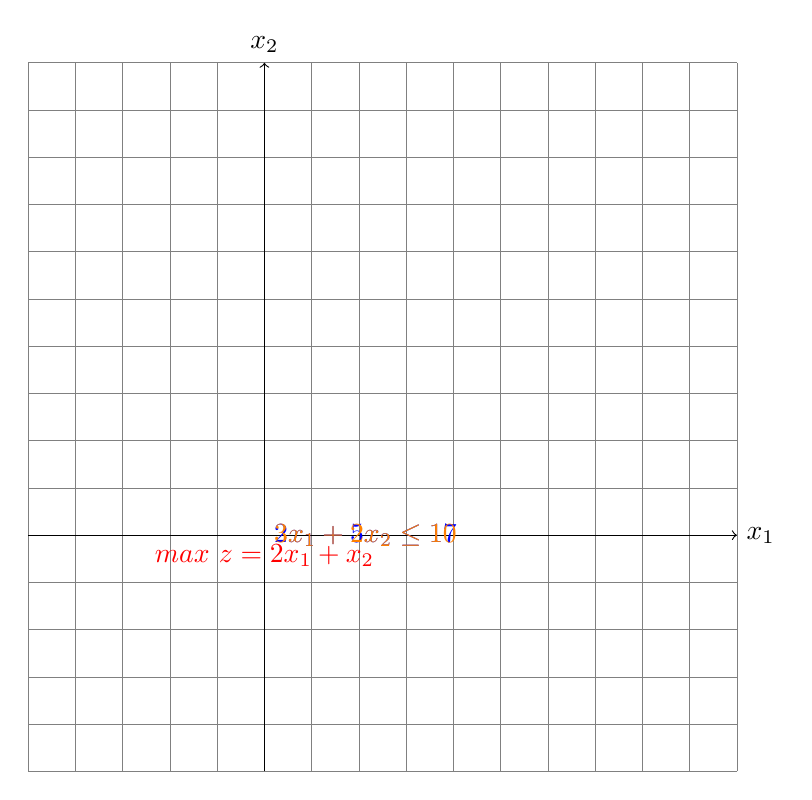
\begin{tikzpicture}[scale = 0.6]

        \filldraw [smooth,draw=gray!20,fill=gray!20] plot[id=f3,domain=0:16.0/11.0]  function {(17.0/5.0) - (2.0/5.0)*x}
            -- (10.0/3.0,0)  -- (0,0) -- cycle;

    \draw[very thin,color=gray] (-5,-5) grid (10, 10);
    \draw[->] plot[id=axeX1] (-5,0) -- (10,0) node[right] {$x_1$};
    \draw[->] plot[id=axeX2] (0,-5) -- (0,10) node[above] {$x_2$};
    
    
    \draw[color=red, domain=-5:2.5, dashed] plot[id=obj] function{-2*x} 
        node[below] {$max\ z = 2x_1 + x_2$};
    \draw[color=blue, domain=-5:10] plot[id=c1] function{(17.0/5.0) - (2.0/5.0)*x} 
        node[right] {$2x_1 + 5x_2 \leq 17$};
    \draw[color=orange, domain=-10.0/3.0:20.0/3.0] plot[id=c2] function{(5.0)-(3.0/2.0)*x} 
        node[right] {$3x_1+2x_2 \leq 10$};
   	
\end{tikzpicture}


\subsection{Résolution graphique}
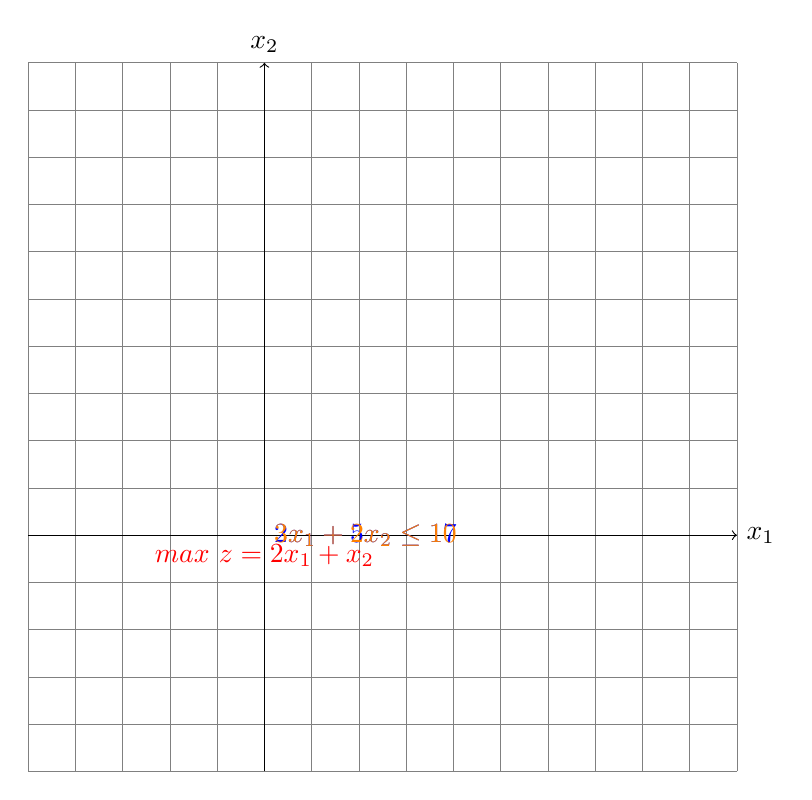
\begin{tikzpicture}[scale = 0.6]

        \filldraw [smooth,draw=gray!20,fill=gray!20] plot[id=f3,domain=0:16.0/11.0]  function {(17.0/5.0) - (2.0/5.0)*x}
            -- (10.0/3.0,0)  -- (0,0) -- cycle;

    \draw[very thin,color=gray] (-5,-5) grid (10, 10);
    \draw[->] plot[id=axeX1] (-5,0) -- (10,0) node[right] {$x_1$};
    \draw[->] plot[id=axeX2] (0,-5) -- (0,10) node[above] {$x_2$};
    
    
    \draw[color=red, domain=-5:2.5, dashed] plot[id=obj] function{-2*x} 
        node[below] {$max\ z = 2x_1 + x_2$};
    \draw[color=red, domain=(-5+1.7):(2.5+1.7), dashed] plot[id=obj] function{17.0/5.0-2*x};
    \draw[color=red, domain=(-5+63.0/22.0):(2.5+63.0/22.0), dashed] plot[id=obj] function{63.0/11.0-2*x};
    \draw[color=red, domain=(-5+10.0/3.0):(2.5+10.0/3.0), dashed] plot[id=obj] function{20.0/3.0-2*x};
        
    \draw[color=blue, domain=-5:10] plot[id=c1] function{(17.0/5.0) - (2.0/5.0)*x} 
        node[right] {$2x_1 + 5x_2 \leq 17$};
    \draw[color=orange, domain=-10.0/3.0:20.0/3.0] plot[id=c2] function{(5.0)-(3.0/2.0)*x)} 
        node[right] {$3x_1+2x_2 \leq 10$};
   	
\end{tikzpicture}

Nous obtenons grâce à la résolution graphique : 
$$ \begin{cases}
x_1 = \frac{10}{3} \\
x_2 = 0 \\
z = \frac{20}{3}
\end{cases} $$


\subsection{Résolution par la méthode du simplexe}
Programme linéaire :
$$
PL_0 \begin{cases}
max\ z(x_1,x_2) = 2x_1 + x_2 \\
 2x_1 + 5x_2 \leq 17 \\
 3x_1 + 2x_2 \leq 10 \\
 x_1, x_2 \geq 0 \\
\end{cases}
$$

Forme standard :
$$
PL_0 \begin{cases}
max\ z(x_1,x_2) = 2x_1 + x_2 \\
 2x_1 + 5x_2 + y_1 = 17 \\
 3x_1 + 2x_2 +y_2 = 10 \\
 x_1, x_2, y_1, y_2 \geq 0 \\
\end{cases}
$$


Tableaux :

$$ \begin{array}{|C{1cm}|C{2cm}|C{1cm} C{1cm} C{1cm} C{1cm}|} \hline
	 &  & 2 & 1 & 0 & 0 \\ \hline
	0 & y_1 = 17 & 2 & 5 & 1 & 0 \\ 
	0 & y_2 = 10 & \textcolor{red}{3} & 2 & 0 & 1 \\ \hline
	 & z = 0 & -2 & -1 & 0 & 0 \\ \hline
 \end{array} $$
 
 $y_2$ sort de la base ; $x_1$ rentre dans la base ; le pivot devient $a_{1,2} = 3$.
 
 $$ \begin{array}{|C{1cm}|C{2cm}|C{1cm} C{1cm} C{1cm} C{1cm}|} \hline
	 &  & 2 & 1 & 0 & 0 \\ \hline
	0 & y_1 = \frac{31}{3} & 0 & \frac{11}{3} & 1 & -\frac{2}{3} \\ 
	2 & x_1 = \frac{10}{3} &1 &  \frac{2}{3} & 0 & \frac{1}{3} \\ \hline
	 & z = \frac{20}{3} & 0 & \frac{1}{3} & 0 & \frac{2}{3} \\ \hline
 \end{array} $$
 
 Tous les coûts réduits sont positifs ou nuls donc le simplexe est fini. La solution correspond bien à celle trouvée graphiquement :
 $$ \begin{cases}
x_1 = \frac{10}{3} \\
x_2 = 0 \\
z = \frac{20}{3}
\end{cases} $$


\subsection{Recherche d'une solution à valeur entière}

\subsubsection{Branch and bound}
Pour la méthode du Branch and bound, nous partons de la solution optimale réelle trouvée précédemment.

\begin{center}
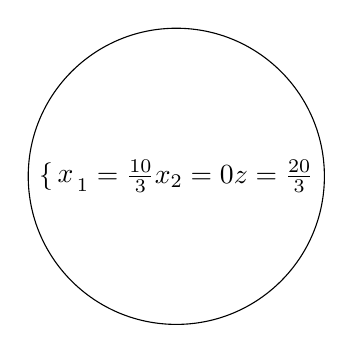
\begin{tikzpicture}[level/.style={sibling distance=7cm,level distance=3.5cm,
			growth parent anchor=south}]
\node [circle,draw] (z){	$ \begin{cases}
						x_1 = \frac{10}{3} \\
						x_2 = 0 \\
					\end{cases}
					z = \frac{20}{3} $}
;
\end{tikzpicture}
\end{center}

Puis nous ajoutons la contrainte $x_1 \leq 3$ pour forcer $x_1$ à être entier.

\begin{center}
\begin{tikzpicture}[level/.style={sibling distance=7cm,level distance=1cm, growth parent anchor=south}]
\node [circle,draw] (z){	$ \begin{cases}
						x_1 = \frac{10}{3} \\
						x_2 = 0 \\
					\end{cases}
					z = \frac{20}{3} $}
child {node [end] (a) {}
	edge from parent 
	node[right] {$x_1 \leq 3$}
	}
child {node [] (a) {}
	edge from parent[draw=none]
	}
;
\end{tikzpicture}
\end{center}

Nous calculons alors les tableaux du simplexe avec la nouvelle contrainte.

$$ \begin{array}{|C{1cm}|C{2cm}|C{1cm} C{1cm} C{1cm} C{1cm} C{1cm}|} \hline
	 &  & 2 & 1 & 0 & 0 & 0 \\ \hline
	0 & y_1 = 17 & 2 & 5 & 1 & 0 & 0 \\ 
	0 & y_2 = 10 & 3 & 2 & 0 & 1 & 0 \\ 
	0 & y_3 = 3 & \textcolor{red}{1} & 0 & 0 & 0 & 1 \\ \hline
	 & z = 0 & -2 & -1 & 0 & 0 & 0 \\ \hline
 \end{array} $$
 
 $y_3$ sort de la base ; $x_1$ rentre dans la base ; le pivot devient $a_{1,3} = 1$.
 
 $$ \begin{array}{|C{1cm}|C{2cm}|C{1cm} C{1cm} C{1cm} C{1cm} C{1cm}|} \hline
	 &  & 2 & 1 & 0 & 0 & 0 \\ \hline
	0 & y_1 = 11 & 0 & 5 & 1 & 0 & -2 \\ 
	0 & y_2 = 1 & 0 & \textcolor{red}{2} & 0 & 1 & -3 \\ 
	2 & x_1 = 3 & 1 & 0 & 0 & 0 & 1 \\ \hline
	 & z = 6 & 0 & -1 & 0 & 0 & 2 \\ \hline
 \end{array} $$

$y_2$ sort de la base ; $x_2$ rentre dans la base ; le pivot devient $a_{2,2} = 2$.

$$ \begin{array}{|C{1cm}|C{2cm}|C{1cm} C{1cm} C{1cm} C{1cm} C{1cm}|} \hline
	 &  & 2 & 1 & 0 & 0 & 0 \\ \hline
	0 & y_1 = \frac{17}{2} & 0 & 0 & 1 & -\frac{5}{2} & 2 \\ 
	1 & x_2 = \frac{1}{2} & 0 & 1 & 0 & \frac{1}{2} & -\frac{3}{2} \\ 
	2 & x_1 = 3 & 1 & 0 & 0 & 0 & 1 \\ \hline
	 & z = \frac{13}{2} & 0 & 0 & 0 & \frac{1}{2} & \frac{1}{2} \\ \hline
 \end{array} $$

Le simplexe est fini, nous ajoutons le résultat à l'arbre de branch and cut.

\begin{center}
\begin{tikzpicture}[level/.style={sibling distance=7cm,level distance=2.5cm,
			growth parent anchor=south}]
\node [circle,draw] (z){	$ \begin{cases}
						x_1 = \frac{10}{3} \\
						x_2 = 0 \\
					\end{cases}
					z = \frac{20}{3} $}
child {node [circle,draw] (a) {	$ \begin{cases}
							x_1 = 3 \\
							x_2 = \frac{1}{2} \\
						\end{cases}
						z = \frac{13}{2} $}
	edge from parent 
	node[left] {$x_1 \leq 3$}
	}
child {node [] (a) {}
	edge from parent[draw=none]
	}
;
\end{tikzpicture}
\end{center}

$x_1$ a bien une valeur entière mais $x_2$ est devenu réel, nous ajoutons donc la contrainte $x_2 \leq 0$. Comme $x_2 \geq 0$ par définition, nous obtenons la solution suivante :

\begin{center}
\begin{tikzpicture}[level/.style={sibling distance=7cm,level distance=2.5cm,
			growth parent anchor=south}]
\node [circle,draw] (z){	$ \begin{cases}
						x_1 = \frac{10}{3} \\
						x_2 = 0 \\
					\end{cases}
					z = \frac{20}{3} $}
child {node [circle,draw] (a) {	$ \begin{cases}
							x_1 = 3 \\
							x_2 = \frac{1}{2} \\
						\end{cases}
						z = \frac{13}{2} $}
	child { node [circle,draw] (b) {$ \begin{cases}
								x_1 = 3 \\
								x_2 = 0 \\
							\end{cases}
							z = 6 $ }
		edge from parent 
		node[left] {$x_2 \leq 0$}
						}
	child {node [] (c) {}
		edge from parent[draw=none]
		}
	edge from parent 
	node[left] {$x_1 \leq 3$}
	}
child {node [] (d) {}
	edge from parent[draw=none]
	}
;
\end{tikzpicture}
\end{center}

Nous obtenons une feuille de l'arbre et une solution entière admissible. Nous devons maintenant développer le reste de l'arbre pour vérifier s'il est possible d'obtenir une meilleure solution entière. Posons donc la contrainte suivante : $x_2 \geq 1$.

\begin{center}
\begin{tikzpicture}[level/.style={sibling distance=7cm,level distance=2.5cm,
			growth parent anchor=south}]
\node [circle,draw] (z){	$ \begin{cases}
						x_1 = \frac{10}{3} \\
						x_2 = 0 \\
					\end{cases}
					z = \frac{20}{3} $}
child {node [circle,draw] (a) {	$ \begin{cases}
							x_1 = 3 \\
							x_2 = \frac{1}{2} \\
						\end{cases}
						z = \frac{13}{2} $}
	child { node [circle,draw] (b) {$ \begin{cases}
								x_1 = 3 \\
								x_2 = 0 \\
							\end{cases}
							z = 6 $ }
		edge from parent 
		node[left] {$x_2 \leq 0$}
						}
	child {node [end] (c) {}
		edge from parent 
		node[right] {$x_2 \geq 1$}
		}
	edge from parent 
	node[left] {$x_1 \leq 3$}
	}
child {node [] (d) {}
	edge from parent[draw=none]
	}
;
\end{tikzpicture}
\end{center}

Afin de trouver une solution, nous appliquons la phase 1 du simplexe dont voici les tableaux.

$$ \begin{array}{|C{1cm}|C{2cm}|C{1cm} C{1cm} C{1cm} C{1cm} C{1cm} C{1cm} C{1cm}|} \hline
	 &  & 0 & 0 & 0 & 0 & 0 & 0 & -1 \\ \hline
	0 & y_1 = 17 & 2 & 5 & 1 & 0 & 0 & 0 & 0 \\ 
	0 & y_2 = 10 & 3 & 2 & 0 & 1 & 0 & 0 & 0 \\ 
	0 & y_3 = 3 & 1 & 0 & 0 & 0 & 1 & 0 & 0 \\ 
	-1 & y_5 = 1 & 0 & \textcolor{red}{1} & 0 & 0 & 0 & -1 & 1 \\ \hline
	 & z = -1 & 0 & -1 & 0 & 0 & 0 & 1 & 0 \\ \hline
 \end{array} $$
 
 $y_5$ sort de la base ; $x_2$ rentre dans la base ; le pivot devient $a_{2,4} = 1$.
 
 $$ \begin{array}{|C{1cm}|C{2cm}|C{1cm} C{1cm} C{1cm} C{1cm} C{1cm} C{1cm} C{1cm}|} \hline
	 &  & 0 & 0 & 0 & 0 & 0 & 0 & -1 \\ \hline
	0 & y_1 = 12 & 2 & 0 & 1 & 0 & 0 & 5 & -5 \\ 
	0 & y_2 = 8 & 3 & 0 & 0 & 1 & 0 & 2 & -2 \\ 
	0 & y_3 = 3 & 1 & 0 & 0 & 0 & 1 & 0 & 0 \\ 
	0 & x_2 = 1 & 0 & 1 & 0 & 0 & 0 & -1 & 1 \\ \hline
	 & z = 0 & 0 & 0 & 0 & 0 & 0 & 0 & 1 \\ \hline
 \end{array} $$

$z = 0$ donc la phase $1$ du simplexe est finie. Passons à la phase $2$...

$$ \begin{array}{|C{1cm}|C{2cm}|C{1cm} C{1cm} C{1cm} C{1cm} C{1cm} C{1cm}|} \hline
	 &  & 2 & 1 & 0 & 0 & 0 & 0 \\ \hline
	0 & y_1 = 12 & 2 & 0 & 1 & 0 & 0 & 5 \\ 
	0 & y_2 = 8 & \textcolor{red}{3} & 0 & 0 & 1 & 0 & 2 \\ 
	0 & y_3 = 3 & 1 & 0 & 0 & 0 & 1 & 0 \\ 
	1 & x_2 = 1 & 0 & 1 & 0 & 0 & 0 & -1 \\ \hline
	 & z = 1 & -2 & 0 & 0 & 0 & 0 & -1 \\ \hline
 \end{array} $$
 
  $y_2$ sort de la base ; $x_1$ rentre dans la base ; le pivot devient $a_{1,2} = 3$.

$$ \begin{array}{|C{1cm}|C{2cm}|C{1cm} C{1cm} C{1cm} C{1cm} C{1cm} C{1cm}|} \hline
	 &  & 2 & 1 & 0 & 0 & 0 & 0 \\ \hline
	0 & y_1 = \frac{20}{3} & 0 & 0 & 1 & -\frac{2}{3} & 0 & \frac{11}{3} \\ 
	2 & x_1 = \frac{8}{3} &1 & 0 & 0 & \frac{1}{3} & 0 & \frac{2}{3} \\ 
	0 & y_3 = \frac{1}{3} & 0 & 0 & 0 & -\frac{1}{3} & 1 & -\frac{2}{3} \\ 
	1 & x_2 = 1 & 0 & 1 & 0 & 0 & 0 & -1 \\ \hline
	 & z = \frac{19}{3} & 0 & 0 & 0 & \frac{2}{3} & 0 & \frac{1}{3} \\ \hline
 \end{array} $$
 
Nous ajoutons la solution obtenue à l'arbre de branch and cut. Comme dans cette solution, $x_1$ n'est pas entier, nous ajoutons également la contrainte : $x_1 \leq 2$.

\begin{center}
\begin{tikzpicture}[level/.style={sibling distance=7cm,level distance=2.5cm,
			growth parent anchor=south}]
\node [circle,draw] (z){	$ \begin{cases}
						x_1 = \frac{10}{3} \\
						x_2 = 0 \\
					\end{cases}
					z = \frac{20}{3} $}
child {node [circle,draw] (a) {	$ \begin{cases}
							x_1 = 3 \\
							x_2 = \frac{1}{2} \\
						\end{cases}
						z = \frac{13}{2} $}
	child { node [circle,draw] (b) {$ \begin{cases}
								x_1 = 3 \\
								x_2 = 0 \\
							\end{cases}
							z = 6 $ }
		edge from parent 
		node[left] {$x_2 \leq 0$}
						}
	child {node [circle,draw] (c) {$ \begin{cases}
								x_1 = \frac{8}{3} \\
								x_2 = 1 \\
							\end{cases}
							z = \frac{19}{3} $ }
		child {node [end] (e) {}
			edge from parent
			node[left] {$x_1 \leq 2$}
			}
		edge from parent 
		node[right] {$x_2 \geq 1$}
		}
	edge from parent 
	node[left] {$x_1 \leq 3$}
	}
child {node [] (d) {}
	edge from parent[draw=none]
	}
;
\end{tikzpicture}
\end{center}

Nous lançons alors la résolution de ce nouveau problème par le simplexe.

$$ \begin{array}{|C{1cm}|C{2cm}|C{1cm} C{1cm} C{1cm} C{1cm} C{1cm} C{1cm}|} \hline
	 &  & 2 & 1 & 0 & 0 & 0 & 0 \\ \hline
	0 & y_1 = 12 & 2 & 0 & 1 & 0 & 0 & 5 \\ 
	0 & y_2 = 8 & 3 & 0 & 0 & 1 & 0 & 2 \\ 
	0 & y_3 = 2 & \textcolor{red}{1} & 0 & 0 & 0 & 1 & 0 \\ 
	1 & x_2 = 1 & 0 & 1 & 0 & 0 & 0 & -1 \\ \hline
	 & z = 1 & -2 & 0 & 0 & 0 & 0 & -1 \\ \hline
 \end{array} $$
 
$y_3$ sort de la base ; $x_1$ rentre dans la base ; le pivot devient $a_{1,3} = 1$.
 
$$ \begin{array}{|C{1cm}|C{2cm}|C{1cm} C{1cm} C{1cm} C{1cm} C{1cm} C{1cm}|} \hline
	 &  & 2 & 1 & 0 & 0 & 0 & 0 \\ \hline
	0 & y_1 = 8 & 0 & 0 & 1 & 0 & -2 & 5 \\ 
	0 & y_2 = 2 & 0 & 0 & 0 & 1 & -3 & \textcolor{red}{2} \\ 
	2 & x_1 = 2 & 1 & 0 & 0 & 0 & 1 & 0 \\ 
	1 & x_2 = 1 & 0 & 1 & 0 & 0 & 0 & -1 \\ \hline
	 & z = 3 & 0 & 0 & 0 & 0 & 2 & -1 \\ \hline
 \end{array} $$
 
$y_2$ sort de la base ; $y_4$ rentre dans la base ; le pivot devient $a_{6,2} = 2$.
 
$$ \begin{array}{|C{1cm}|C{2cm}|C{1cm} C{1cm} C{1cm} C{1cm} C{1cm} C{1cm}|} \hline
	 &  & 2 & 1 & 0 & 0 & 0 & 0 \\ \hline
	0 & y_1 = 3 & 0 & 0 & 1 & -\frac{5}{2} & \frac{11}{2} & 0 \\ 
	0 & y_4 = 1 & 0 & 0 & 0 & \frac{1}{2} & -\frac{3}{2} & 1 \\ 
	2 & x_1 = 2 & 1 & 0 & 0 & 0 & 1 & 0 \\ 
	1 & x_2 = 2 & 0 & 1 & 0 & \frac{1}{2} & -\frac{3}{2} & 0 \\ \hline
	 & z = 6 & 0 & 0 & 0 & \frac{1}{2} & \frac{1}{2} & 0 \\ \hline
 \end{array} $$

La résolution par le simplexe est finie et nous obtenons une solution entière égale à celle précédemment trouvée. Cette solution est donc une feuille de l'arbre ; nous remontons d'un niveau et ajoutons la contrainte $x_1 \geq 4$.

Nous remarquons que cette contrainte force $x_1$ à violer la deuxième contrainte du problème originel : $3x_1 + 2x_2 \leq 10$. En effet $3 \times 4 > 10$, cette contrainte ne mène donc à aucune nouvelle solution et l'arbre de branch and cut est terminé.

Nous avons donc trouvé deux solutions optimales entières au problème :\\
$ \begin{cases}
	x_1 = 2 \\
	x_2 = 2 \\
	z = 6
\end{cases} $
et
$ \begin{cases}
	x_1 = 3 \\
	x_2 = 0 \\
	z = 6
\end{cases}$

 
\begin{center}
\begin{tikzpicture}[level/.style={sibling distance=7cm,level distance=2.5cm,
			growth parent anchor=south}]
\node [circle,draw] (z){	$ \begin{cases}
						x_1 = \frac{10}{3} \\
						x_2 = 0 \\
					\end{cases}
					z = \frac{20}{3} $}
child {node [circle,draw] (a) {	$ \begin{cases}
							x_1 = 3 \\
							x_2 = \frac{1}{2} \\
						\end{cases}
						z = \frac{13}{2} $}
	child { node [circle,draw] (b) {$ \begin{cases}
								x_1 = 3 \\
								x_2 = 0 \\
							\end{cases}
							z = 6 $ }
		edge from parent 
		node[left] {$x_2 \leq 0$}
						}
	child {node [circle,draw] (c) {$ \begin{cases}
								x_1 = \frac{8}{3} \\
								x_2 = 1 \\
							\end{cases}
							z = \frac{19}{3} $ }
		child {node [circle,draw] (e)  {$ \begin{cases}
									x_1 = 2 \\
									x_2 = 2 \\
								\end{cases}
								z = 6 $ }
			edge from parent
			node[left] {$x_1 \leq 2$}
			}
		edge from parent 
		node[right] {$x_2 \geq 1$}
		}
	edge from parent 
	node[left] {$x_1 \leq 3$}
	}
child {node [end] (d) {}
	edge from parent
	node[left] {$x_1 \geq 4$}
	}
;
\end{tikzpicture}
\end{center}


\subsubsection{Coupes de Gomory}

La méthode des coupes de Gomory nécessite une solution optimale réelle, nous partons donc de celle trouvée précédemment :
$$ \begin{cases}
x_1 = \frac{10}{3} \\
x_2 = 0 \\
z = \frac{20}{3}
\end{cases} $$

et du dernier tableau du simplexe associé :

$$ \begin{array}{|C{1cm}|C{2cm}|C{1cm} C{1cm} C{1cm} C{1cm}|} \hline
	 &  & 2 & 1 & 0 & 0 \\ \hline
	0 & y_1 = \frac{31}{3} & 0 & \frac{11}{3} & 1 & -\frac{2}{3} \\ 
	2 & x_1 = \frac{10}{3} &1 &  \frac{2}{3} & 0 & \frac{1}{3} \\ \hline
	 & z = \frac{20}{3} & 0 & \frac{1}{3} & 0 & \frac{2}{3} \\ \hline
 \end{array} $$

Nous avons choisi la deuxième ligne du tableau pour en déduire la contrainte de Gomory suivante :
 $$ <\frac{2}{3}>x_2 + <\frac{1}{3}>y_2 \geq <\frac{10}{3}> $$
 $$ \Leftrightarrow $$
 $$ \frac{2}{3}x_2 + \frac{1}{3}y_2 \geq \frac{1}{3} $$
Nous devons maintenant l'exprimer uniquement en fonction de $x_1$ et $x_2$. Remplaçons donc $y_2$ par son équivalent dans la contrainte 2, cela donne :
$$ x_1 \leq 3 $$
Nous devons maintenant utiliser le simplexe pour résoudre le problème avec la nouvelle contrainte. L'ayant déjà fait lors de la question précédente, sautons directement au résultat :

$ \begin{cases}
	x_1 = 3 \\
	x_2 = \frac{1}{2} \\
	z = \frac{13}{2}
\end{cases} $

et le dernier tableau associé :

$$ \begin{array}{|C{1cm}|C{2cm}|C{1cm} C{1cm} C{1cm} C{1cm} C{1cm}|} \hline
	 &  & 2 & 1 & 0 & 0 & 0 \\ \hline
	0 & y_1 = \frac{17}{2} & 0 & 0 & 1 & -\frac{5}{2} & 2 \\ 
	1 & x_2 = \frac{1}{2} & 0 & 1 & 0 & \frac{1}{2} & -\frac{3}{2} \\ 
	2 & x_1 = 3 & 1 & 0 & 0 & 0 & 1 \\ \hline
	 & z = \frac{13}{2} & 0 & 0 & 0 & \frac{1}{2} & \frac{1}{2} \\ \hline
 \end{array} $$

Nous choisissons la ligne 2 du tableau pour exprimer la contrainte de Gomory :
 $$ <\frac{1}{2}>y_2 + <-\frac{3}{2}>y_3 \geq <\frac{1}{2}> $$
 $$ \Leftrightarrow $$
 $$ \frac{1}{2}y_2 + \frac{1}{2}y_3 \geq \frac{1}{2} $$
Nous devons maintenant l'exprimer uniquement en fonction de $x_1$ et $x_2$. Remplaçons donc $y_2$ par son équivalent dans la contrainte 2, cela donne :
$$ x_2 \leq 2y_3 $$
Remplaçons maintenant $y_3$ par son équivalent dans la contrainte 3, cela donne :
$$ 2x_1 + x_2 \leq 6 $$

Résolvons le problème avec cette contrainte en plus :
$$ \begin{array}{|C{1cm}|C{2cm}|C{1cm} C{1cm} C{1cm} C{1cm} C{1cm} C{1cm}|} \hline
	 &  & 2 & 1 & 0 & 0 & 0 & 0 \\ \hline
	0 & y_1 = 17 & 2 & 5 & 1 & 0 & 0 & 0 \\ 
	0 & y_2 = 10 & 3 & 2 & 0 & 1 & 0 & 0 \\ 
	0 & y_3 = 3 & 1 & 0 & 0 & 0 & 1 & 0 \\ 
	0 & y_4 = 6 & \textcolor{red}{2} & 1 & 0 & 0 & 0 & 1 \\ \hline
	 & z = 0 & -2 & -1 & 0 & 0 & 0 & 0 \\ \hline
 \end{array} $$
 
 $y_4$ sort de la base ; $x_1$ rentre dans la base ; le pivot devient $a_{1,4} = 2$.
 
 $$ \begin{array}{|C{1cm}|C{2cm}|C{1cm} C{1cm} C{1cm} C{1cm} C{1cm} C{1cm}|} \hline
	 &  & 2 & 1 & 0 & 0 & 0 & 0 \\ \hline
	0 & y_1 = 11 & 0 & 4 & 1 & 0 & 0 & -1 \\ 
	0 & y_2 = 1 & 0 & \frac{1}{2} & 0 & 1 & 0 & -\frac{3}{2} \\ 
	0 & y_3 = 0 & 0 & -\frac{1}{2} & 0 & 0 & 1 & -\frac{1}{2}  \\ 
	2 & x_1 = 3 & 1 & \frac{1}{2} & 0 & 0 & 0 & \frac{1}{2} \\ \hline
	 & z = 6 & 0 & 0 & 0 & 0 & 0 & 1 \\ \hline
 \end{array} $$
 
Et voici donc la solution finale de la méthode des coupes de Gomory :
$ \begin{cases}
	x_1 = 3 \\
	x_2 = 0 \\
	z = 6
\end{cases} $.


